% !TEX root = ../main.tex

\chapter{插图和表格}

\section{三线表}

三线表是《撰写手册》推荐使用的格式，如表~\ref{tab:exampletable}。

\begin{table}
  \centering
  \caption{表号和表题在表的正上方}
%  \bicaption{表号和表题在表的正上方}{Test table 1}
  \label{tab:exampletable}
  \begin{tabular}{cl}
    \toprule
    类型   & \multicolumn{1}{c}{描述}               \\
    \midrule
    挂线表 & 挂线表也称系统表、组织表，用于表现系统结构 \\
    无线表 & 无线表一般用于设备配置单、技术参数列表等   \\
    卡线表 & 卡线表有完全表，不完全表和三线表三种       \\
    \bottomrule
  \end{tabular}
\end{table}


如果有表注，推荐使用 \pkg{threeparttable}。这样可以与表格对齐，满足部分评审老师的要求。

\begin{table}
  \centering
  \begin{threeparttable}
    \caption{带表注的表格}
%    \bicaption{带表注的表格}{Test table 2}
    \label{tab:tablewithnotes}
    \begin{tabular}{cl}
      \toprule
      类型   & \multicolumn{1}{c}{描述}              \\
      \midrule
      挂线表 & 挂线表也称系统表、组织表，用于表现系统结构 \\
      无线表 & 无线表一般用于设备配置单、技术参数列表等   \\
      卡线表 & 卡线表有完全表，不完全表和三线表三种       \\
      \bottomrule
    \end{tabular}
    \begin{tablenotes}[flushleft]
      \item 注：表注分两种，第一种是对全表的注释，用不加阿拉伯数字排在表的下边，
      前面加“注：”；第二种是和表内的某处文字或数字相呼应的注，
      在表里面用带圈的阿拉伯数字在右上角标出，然后在表下面用同样的圈码注出来
    \end{tablenotes}
  \end{threeparttable}
\end{table}


编制表格应简单明了，表达一致，明晰易懂，表文呼应、内容一致。
排版时表格字号略小，或变换字体，尽量不分页，尽量不跨节。
表格太大需要转页时，需要在续表上方注明“续表”，表头页应重复排出。



\section{插图}

有的同学可能听说“\LaTeX{} 只能使用 eps 格式的图片”，甚至把 jpg 格式转为 eps。
事实上，这种做法已经过时。
而且每次编译时都要要调用外部工具解析 eps，导致降低编译速度。
所以我们推荐矢量图直接使用 pdf 格式，位图使用 jpeg 或 png 格式。

\begin{figure}[ht]
  \centering
  
\includegraphics[width=0.38\textwidth]{sysu-logo.pdf}
  \caption{图号、图题置于图的下方}
%  \bicaption{图号、图题置于图的下方}{Test figure 1}
  \label{fig:confusion}
  \figurenote{若有图注，图注置于图题下方。
    多个图注则须顺序编号，注序左缩进2字，与注文之间空一字符，续行悬挂缩进左对齐，两端对齐。
    注文的字数较少且是短语时，末尾不可加标点，多个图注可以在同一行通过自由选取字符空格将各个图注间隔开来；
    注文的字数较多或者甚至需要用句子说明时，该图注可以独立成行。
  }
\end{figure}

关于图片的并排，推荐使用较新的 \pkg{subcaption} 宏包，
不建议使用 \pkg{subfigure} 或 \pkg{subfig} 等宏包。下面给出几个子图的例子。

\begin{figure}[h]%文中的Grid-LSTM模型做的语义图像分割的例子
    \centering
    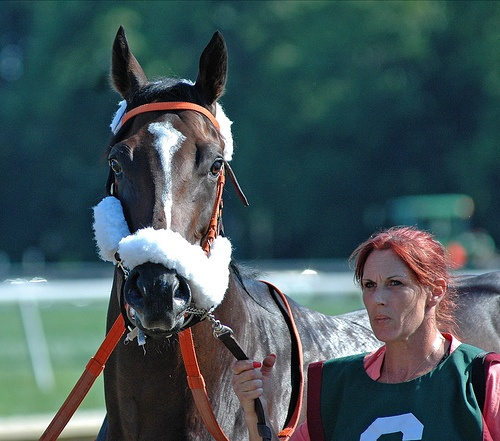
\includegraphics[width=.2\textwidth,height=.15\textwidth]{figures/chap02/example/2007_000799.jpg}
    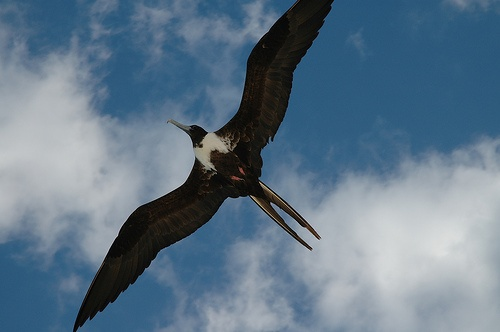
\includegraphics[width=.2\textwidth,height=.15\textwidth]{figures/chap02/example/2007_002094.jpg}
    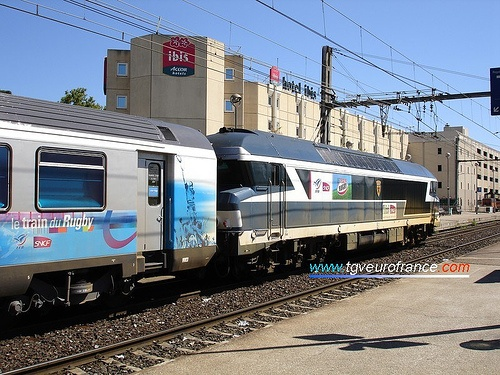
\includegraphics[width=.2\textwidth,height=.15\textwidth]{figures/chap02/example/2007_004483.jpg}
    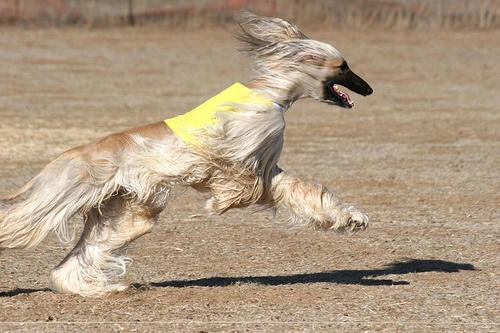
\includegraphics[width=.2\textwidth,height=.15\textwidth]{figures/chap02/example/2007_003194.jpg}
    \\
    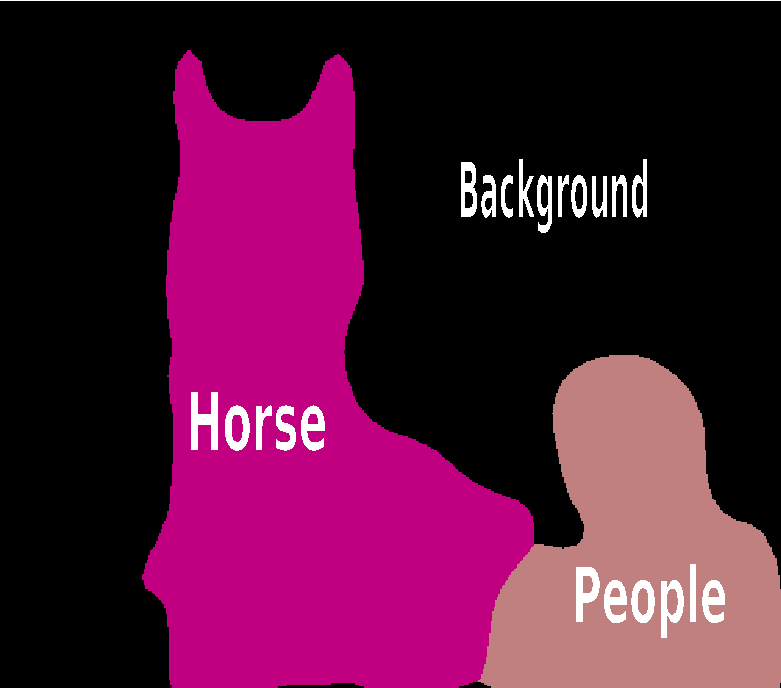
\includegraphics[width=.2\textwidth,height=.15\textwidth]{figures/chap02/example/2007_000799.pdf}
    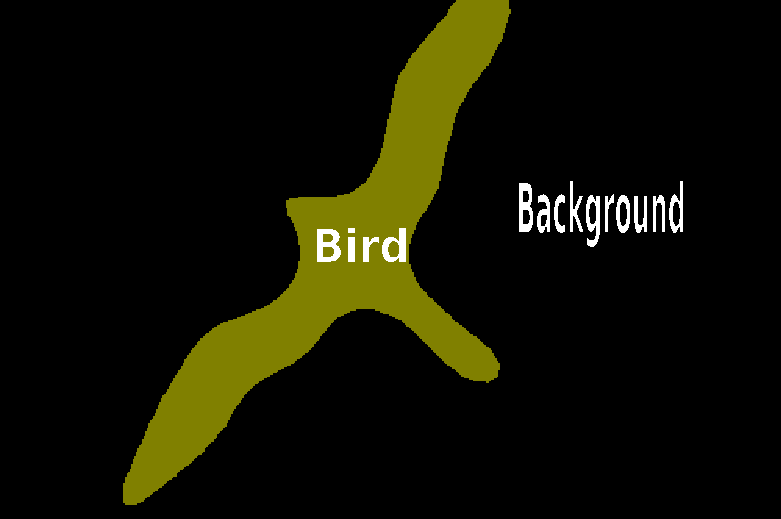
\includegraphics[width=.2\textwidth,height=.15\textwidth]{figures/chap02/example/2007_002094.pdf}
    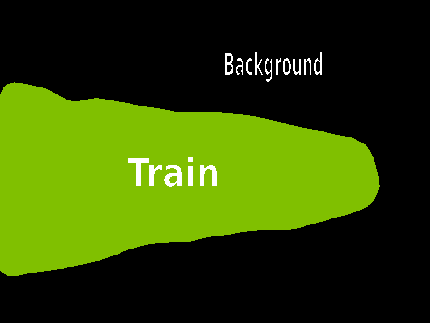
\includegraphics[width=.2\textwidth,height=.15\textwidth]{figures/chap02/example/2007_004483.pdf}
    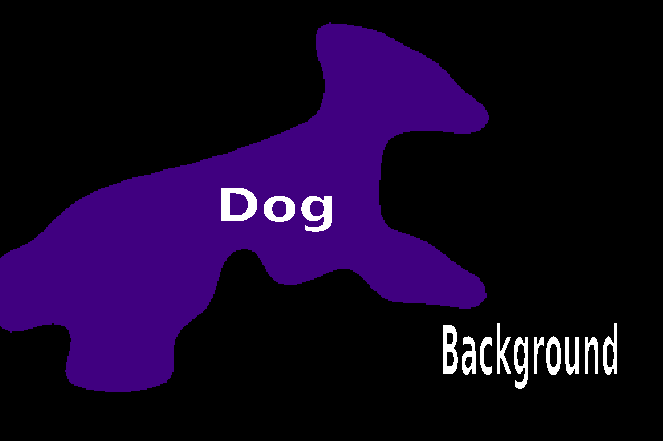
\includegraphics[width=.2\textwidth,height=.15\textwidth]{figures/chap02/example/2007_003194.pdf}
    \caption{并排的多张图像}
    \label{fig:multi-image-example1}
\end{figure}

\begin{figure}[h]
    \centering
    \makebox[0.11\textwidth]{\scriptsize 图像}
    \enspace
    \makebox[0.11\textwidth]{\scriptsize 真值}
    \enspace
    \makebox[0.11\textwidth]{\scriptsize CNN+5LSTM\textbf{1}}
    \enspace\thinspace
    \makebox[0.11\textwidth]{\scriptsize CNN+5LSTM\textbf{2}}
    \enspace\thinspace
    \makebox[0.11\textwidth]{\scriptsize CNN+5LSTM\textbf{3}}
    \enspace\thinspace
    \makebox[0.11\textwidth]{\scriptsize CNN+5LSTM\textbf{4}}
    \enspace\thinspace
    \makebox[0.11\textwidth]{\scriptsize CNN+5LSTM\textbf{5}}\\
    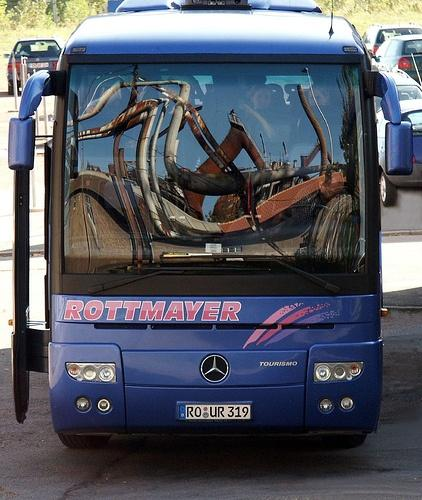
\includegraphics[width=0.11\textwidth]{figures/chap02/improvement/2007_000663.jpg}
    \enspace\thinspace %\hfill
    
\includegraphics[width=0.11\textwidth]{figures/chap02/improvement/2007_000663.png}
    \enspace\thinspace
    
\includegraphics[width=0.11\textwidth]{figures/chap02/improvement/2007_000663_1.png}
    \enspace\thinspace
    
\includegraphics[width=0.11\textwidth]{figures/chap02/improvement/2007_000663_2.png}
    \enspace\thinspace
    
\includegraphics[width=0.11\textwidth]{figures/chap02/improvement/2007_000663_3.png}
    \enspace\thinspace
    
\includegraphics[width=0.11\textwidth]{figures/chap02/improvement/2007_000663_4.png}
    \enspace\thinspace
    
\includegraphics[width=0.11\textwidth]{figures/chap02/improvement/2007_000663_5.png}
    \enspace\thinspace
    \caption{并排的多张图像加各自的注解}
    \label{fig:improvement}
\end{figure}

\begin{figure}[h] % image examples & compare
    \begin{subfigure}{0.55\textwidth}
        \makebox[0.18\textwidth]{\scriptsize Grid-5LSTM}
        \makebox[0.18\textwidth]{\scriptsize FCN-8s}
        \makebox[0.18\textwidth]{\scriptsize SDS}
        \makebox[0.18\textwidth]{\scriptsize 真值}
        \makebox[0.18\textwidth]{\scriptsize 图像} \\
        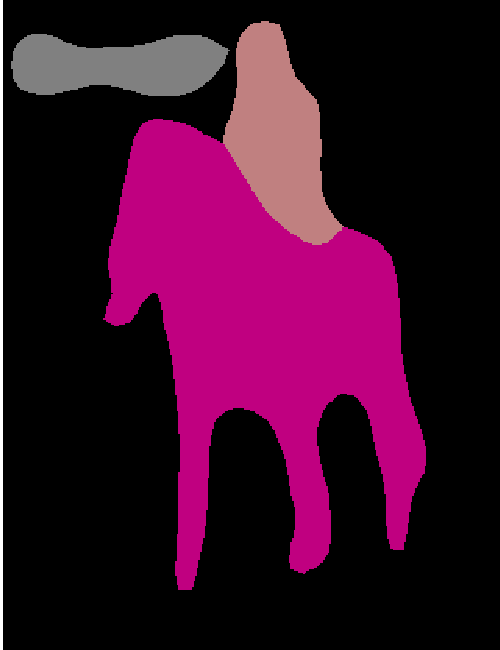
\includegraphics[width=0.18\textwidth]{figures/chap02/compare/my_horse.pdf}
        
\includegraphics[width=0.18\textwidth]{figures/chap02/compare/fcn_horse.png}
        
\includegraphics[width=0.18\textwidth]{figures/chap02/compare/sds_horse.png}
        
\includegraphics[width=0.18\textwidth]{figures/chap02/compare/gt_horse.pdf}
        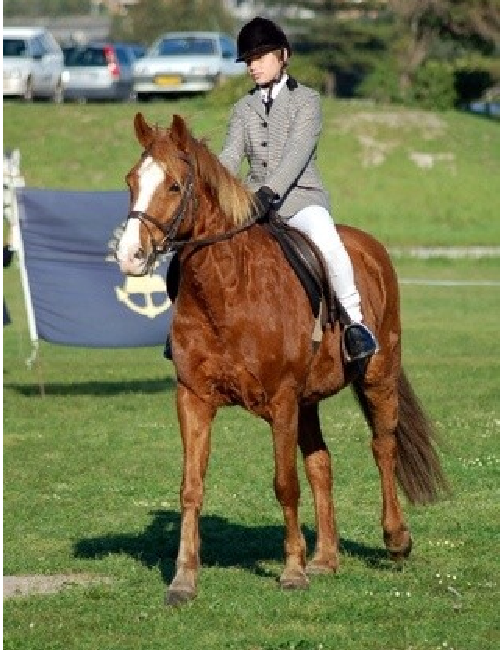
\includegraphics[width=0.18\textwidth]{figures/chap02/compare/im_horse.pdf}
        \\
        
\includegraphics[width=0.18\textwidth]{figures/chap02/compare/my_motor.png}
        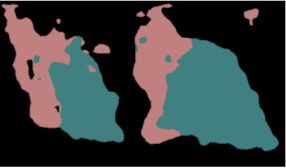
\includegraphics[width=0.18\textwidth]{figures/chap02/compare/fcn_motor.png}
        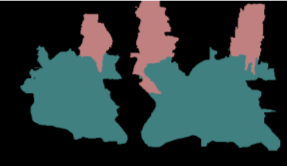
\includegraphics[width=0.18\textwidth]{figures/chap02/compare/sds_motor.png}
        
\includegraphics[width=0.18\textwidth]{figures/chap02/compare/2007_005173.png}
        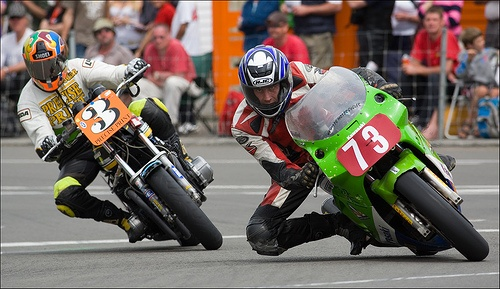
\includegraphics[width=0.18\textwidth]{figures/chap02/compare/2007_005173.jpg}
        \\
        
\includegraphics[width=0.18\textwidth]{figures/chap02/compare/my_sheep.pdf}
        
\includegraphics[width=0.18\textwidth]{figures/chap02/compare/fcn_sheep.png}
        
\includegraphics[width=0.18\textwidth]{figures/chap02/compare/sds_sheep.png}
        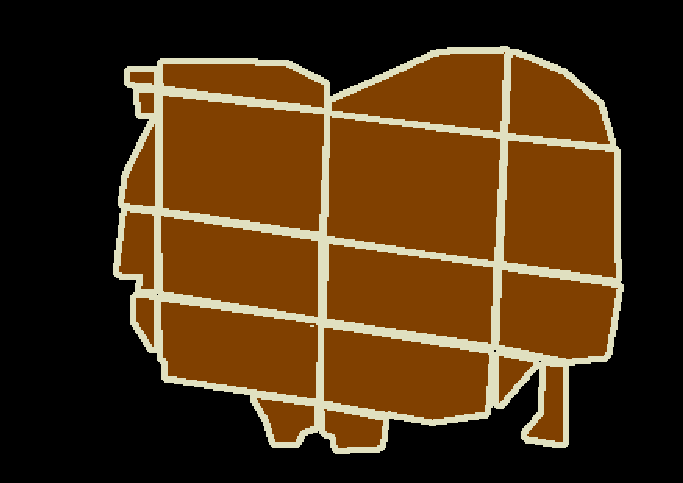
\includegraphics[width=0.18\textwidth]{figures/chap02/compare/gt_sheep.pdf}
        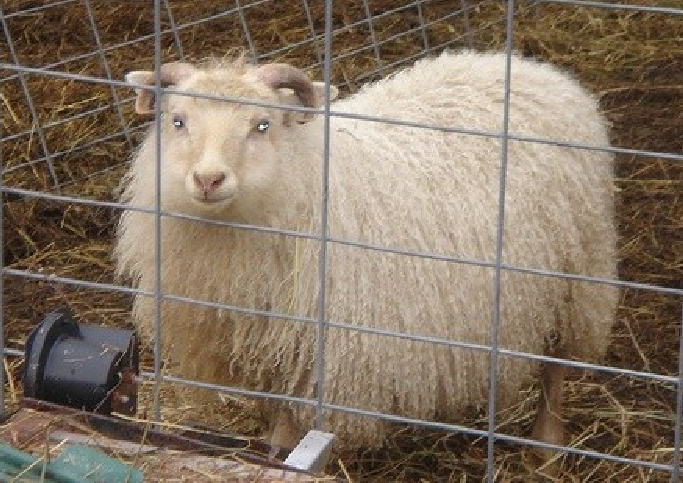
\includegraphics[width=0.18\textwidth]{figures/chap02/compare/im_sheep.pdf}
        \\
        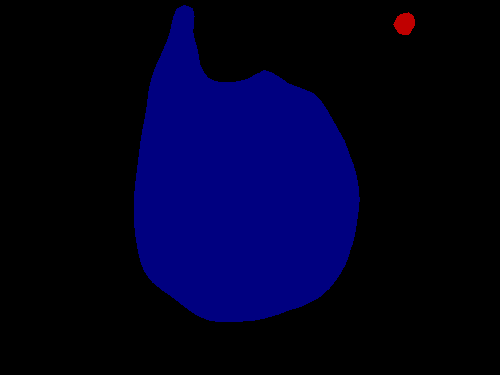
\includegraphics[width=0.18\textwidth]{figures/chap02/compare/my_boat.png}
        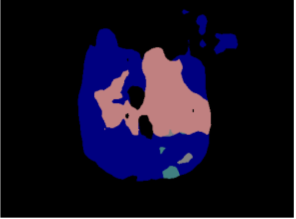
\includegraphics[width=0.18\textwidth]{figures/chap02/compare/fcn_boat.png}
        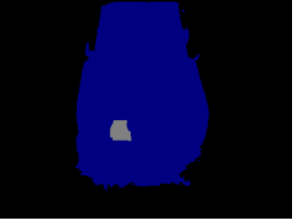
\includegraphics[width=0.18\textwidth]{figures/chap02/compare/sds_boat.png}
        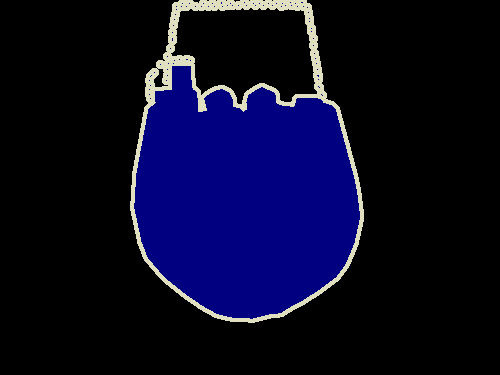
\includegraphics[width=0.18\textwidth]{figures/chap02/compare/2007_004241.png}
        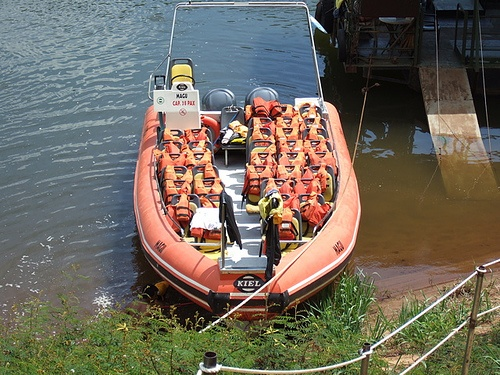
\includegraphics[width=0.18\textwidth]{figures/chap02/compare/2007_004241.jpg}
        \label{fig:compare1}
    \end{subfigure}
    \begin{subfigure}{0.4\textwidth}
        \centering
        %		\makebox[0.3\textwidth]{} \\
        %		\makebox[0.3\textwidth]{} \\
        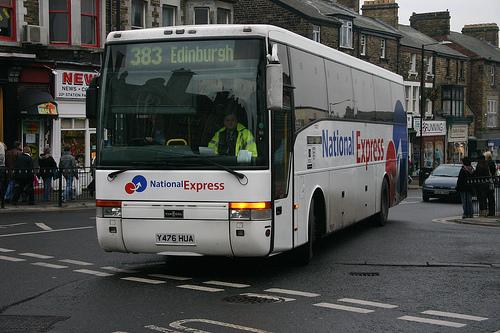
\includegraphics[width=0.25\textwidth]{figures/chap02/compare/2010_005284.jpg}
        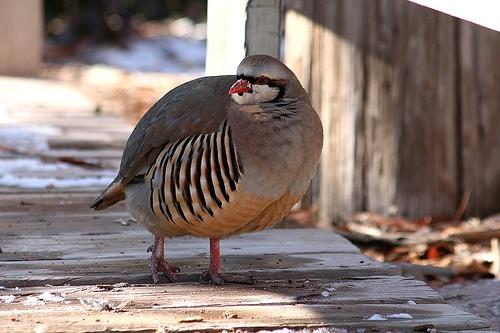
\includegraphics[width=0.25\textwidth]{figures/chap02/compare/2007_003349.jpg}
        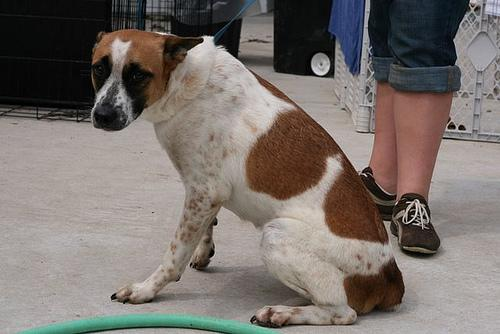
\includegraphics[width=0.25\textwidth]{figures/chap02/compare/2009_004507.jpg}
        \\
        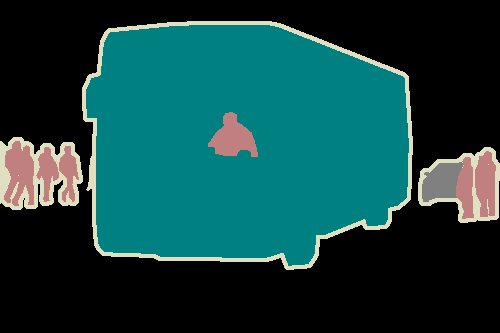
\includegraphics[width=0.25\textwidth]{figures/chap02/compare/2010_005284.png}
        
\includegraphics[width=0.25\textwidth]{figures/chap02/compare/2007_003349.png}
        
\includegraphics[width=0.25\textwidth]{figures/chap02/compare/2009_004507.png} \\
        
\includegraphics[width=0.25\textwidth]{figures/chap02/compare/zoom_bus.png}
        
\includegraphics[width=0.25\textwidth]{figures/chap02/compare/zoom_bird.png}
        
\includegraphics[width=0.25\textwidth]{figures/chap02/compare/zoom_dog.png} \\
        
\includegraphics[width=0.25\textwidth]{figures/chap02/compare/deeplab_bus.png}
        
\includegraphics[width=0.25\textwidth]{figures/chap02/compare/deeplab_bird.png}
        
\includegraphics[width=0.25\textwidth]{figures/chap02/compare/deeplab_dog.png} \\
        
\includegraphics[width=0.25\textwidth]{figures/chap02/compare/my_bus.png}
        
\includegraphics[width=0.25\textwidth]{figures/chap02/compare/my_bird.png}
        
\includegraphics[width=0.25\textwidth]{figures/chap02/compare/my_dog.png}
        \label{fig:compare2}
    \end{subfigure}
    \caption{复杂的两列图象的插入}
    \label{fig:complex}
\end{figure}


\section{算法环境}

模板中使用 \pkg{algorithm2e} 宏包实现算法环境。关于该宏包的具体用法，
请阅读宏包的官方文档。


\label{sec:algorithm}
\begin{algorithm}[ht]
    \KwIn{$m$个训练样本}
    \lFor{$l=1$ \emph{\KwTo} $n_l$}{
        初始化：$\Delta \mathbf{W}^{(l)}=0$，$\Delta \mathbf{b}^{(l)}=0$}
    \ForEach{训练样本}{
        \lFor{$l=1$ \emph{\KwTo} $n_l-1$}{
            前向传播：$\mathbf{z}^{(l+1)}=\mathbf{W}^la^l+\mathbf{b}^l$,$\mathbf{a}^{(l+1)}=f(\mathbf{z}^{(l+1)})$}
        输出误差计算：$\delta^{(n_l)} = \frac{\partial}{\partial \mathbf{z}^{(n_l)}} J(\mathbf{W},\mathbf{b};\mathbf{x},y)$\;
        \lFor{$l=n_l-1$ \emph{\KwTo} $1$}{
            后向传播：$\delta^{(l)} = \bigl((\mathbf{W}^{(l)})^T \delta^{(l+1)}\bigr)f'(\mathbf{z}^{(l)})$}
        \ForAll{层l}{
            计算梯度：$\nabla_{\mathbf{W}^{(l)}}J(\mathbf{W},\mathbf{b};\mathbf{x},y)=\delta^{(l+1)}(\mathbf{a}^{(l)})^T$ \\
            \hspace{60pt}$\nabla_{\mathbf{b}^{(l)}}J(\mathbf{W},\mathbf{b};\mathbf{x},y)=\delta^{(l+1)}$\;
            累加梯度：$\Delta \mathbf{W}^{(l)} \leftarrow \Delta \mathbf{W}^{(l)} + \nabla_{\mathbf{W}^{(l)}}J(\mathbf{W},\mathbf{b};\mathbf{x},y)$; \\
            \hspace{60pt}$\Delta \mathbf{b}^{(l)} \leftarrow \Delta \mathbf{b}^{(l)} + \nabla_{\mathbf{b}^{(l)}}J(\mathbf{W},\mathbf{b};\mathbf{x},y)$\;
        }
    }
    \ForAll{层$l$}{
        更新权重：$\mathbf{W}^{(l)} \leftarrow \mathbf{W}^{(l)} - \alpha \biggl[\frac 1m \Delta \mathbf{W}^{(l)}\biggr]$ \\
        \hspace{60pt} $\mathbf{b}^{(l)} \leftarrow \mathbf{b}^{(l)} - \alpha \biggl[\frac 1m \Delta \mathbf{b}^{(l)}\biggr]$
    }
    \caption{梯度下降算法}
    \label{algo:sgd}
\end{algorithm}

本模板可以在论文中插入算法，但是插入大段的代码是不明智的。
然而这并不妨碍有的同学选择这么做，对于这些同学，建议用 \pkg{listings} 宏包。例如，在论文中插入代码片段的效果为：

\begin{lstlisting}[
 numbers=left,
 basicstyle=\ttfamily,
 breaklines=true,
 keywordstyle=\color{SeaGreen4},
 caption=CPP example,
 language=C++
]
#include <iostream>
int main()
{
    ::std::cout << "hello world" << ::std::endl;
    return 0;
}
\end{lstlisting}

也可在行内插入代码片段，例如：Python中重载加法运算符的函数为\lstinline[language=Python,keywordstyle=\color{SeaGreen4}]{__add__}。
此外，还可直接插入代码文件，例如插入\texttt{./code/demo.cpp}的效果为：

\lstinputlisting[
 basicstyle=\ttfamily,
 breaklines=true,
 keywordstyle=\color{SeaGreen4},
 language=C++
]{code/demo.cpp}
